\documentclass[tikz, border=1mm]{standalone}

\begin{document}
	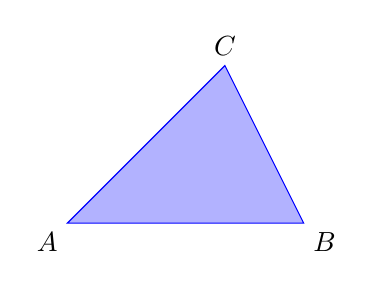
\begin{tikzpicture}
		% Define coordinates
		\coordinate (A) at (0,0);
		\coordinate (B) at (3,0);
		\coordinate (C) at (2,2);
		
		% Draw triangle and fill with blue
		\draw[blue, fill=blue!30] (A) -- (B) -- (C) -- cycle;
		
		% Label vertices
		\node[below left] at (A) {$A$};
		\node[below right] at (B) {$B$};
		\node[above] at (C) {$C$};
	\end{tikzpicture}
\end{document}